\section{評価}
\label{sec:Evaluation}
本章では,提案手法の有効性を確認するために行った評価について述べる.評価では,単回帰分析において,1台での集中学習を行う場合,TCP/IPによる通信を用いた分散学習を行う場合,提案手法を用いた分散学習を行う場合の実行時間を比較した.

\subsection{評価用プログラム}
評価用プログラムとして単回帰分析を行うプログラムを作成した.単回帰分析とは,与えられたデータを用いて$y = ax + b$の傾き$a$と切片$b$を求める問題である.パラメータの最適化には確率的勾配降下法(Stochastic Gradient Descent, SGD)を用いた.確率的勾配降下法とは,データをランダムに選んで以下の更新を繰り返し,$f$を最小化するアルゴリズムである.なお,パラメータを$w$,学習率を$\alpha$,目的関数を$f$とする.

\begin{equation}
  w \leftarrow w - \alpha \nabla f(w)
\end{equation}

複数台の計算機で分散して学習を行う場合はパラメータの集約が必要となる.パラメータの集約にはGossip Learning \cite{Gossip1}, \cite{Gossip2} を用いた.Gossip Learningにおいて,各計算機は確率的勾配降下法によってパラメータを更新する.そして,定期的にランダムに選んだ他の計算機と通信し,パラメータの平均を計算する.このようなパラメータの更新を繰り返していくことによって学習が進む.

このプログラムは1台での集中学習を行うもの,TCP/IPによる通信を用いた分散学習を行うもの,提案手法を用いた分散学習を行うものの3種類を作成した.

\subsection{評価環境}
評価で用いたネットワーク構成を図\ref{fig:Evaluation}に示す.計算機をメッシュネットワークで接続し,それぞれの計算機で評価用プログラムを動作させた.なお,評価で用いた計算機の性能は事前実験1で用いたもの(表\ref{tab:MachineSpec})と同じである.

\begin{figure}[htb]
  \centering
  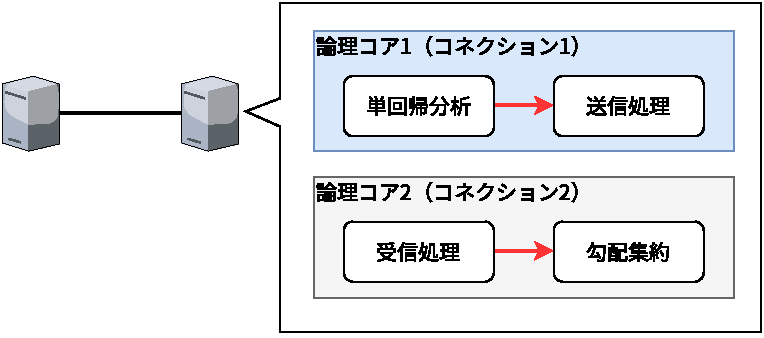
\includegraphics[width=\columnwidth]{pictures/EvaluationNetwork.pdf}
  \caption{評価で用いたネットワーク構成}
  \label{fig:Evaluation}
\end{figure}

\subsection{評価結果・考察}
評価結果を図\ref{fig:EvaluationResult}に示す.このグラフの横軸は左から1台での集中学習の場合,TCP/IPによる通信を用いた2台での分散学習の場合,提案手法を用いた2台での分散学習の場合を表しており,縦軸は実行時間を表している.グラフより,提案手法を用いた2台での分散学習の実行時間は,1台での集中学習の50\%程度,TCP/IPによる通信を用いた2台での分散学習の83\%程度であることがわかる.よって,分散計算環境において,DPDKによるL2通信を用いることとDPDKのRun-to-Completionモデルで処理を行うことは有効であると考える.

\begin{figure}[htb]
  \centering
  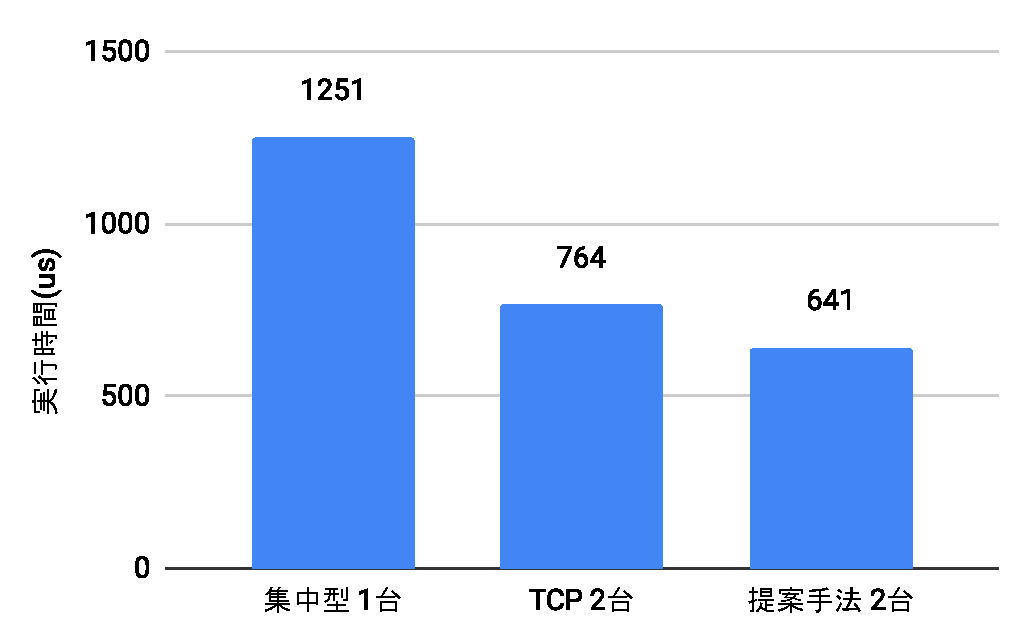
\includegraphics[width=\columnwidth]{pictures/EvaluationResult.pdf}
  \caption{評価結果}
  \label{fig:EvaluationResult}
\end{figure}
